% !TeX program = xelatex
\documentclass[10pt,a4paper,twocolumn]{article}
\usepackage[top=19mm,bottom=20mm,left=18mm,right=18mm,columnsep=6mm]{geometry}
\usepackage{fontspec}
\setmainfont{Latin Modern Roman}
\usepackage{amsmath,amssymb,booktabs,array,graphicx,microtype}
\usepackage[font=small,labelfont=bf]{caption}
\usepackage[hidelinks]{hyperref}
\usepackage{url}
\usepackage{etoolbox}
\usepackage{balance}
\apptocmd{\thebibliography}{\setlength{\itemsep}{0pt}\setlength{\parsep}{0pt}}{}{}
\setlength{\parindent}{1em}
\setlength{\parskip}{0pt}
\setlength{\emergencystretch}{1.5em}
\setlength{\textfloatsep}{11pt plus 2pt minus 2pt}
\setlength{\floatsep}{9pt plus 2pt minus 2pt}
\setcounter{dbltopnumber}{2}
\renewcommand{\dbltopfraction}{0.78}
\raggedbottom
\clubpenalty=10000
\widowpenalty=10000
\brokenpenalty=10000
\newcommand{\GR}{\mathrm{GR{+}P}}
\newcommand{\RGR}{\mathrm{RGR{+}P}}
\newcommand{\AuthorNames}{Nguyen Minh Tung}
\newcommand{\StudentIDs}{A0343185A}
\newcommand{\RepositoryURL}{https://github.com/junghyukie/Final_Assignment}

\hypersetup{
    pdfauthor={Nguyen Minh Tung},
    pdftitle={Evaluating Feedback in LLM-Guided Heuristic Evolution for Minimum Weighted Dominating Set}
}
\title{
    Evaluating Feedback in LLM-Guided Heuristic Evolution\\
    \large for Minimum Weighted Dominating Set
}
\author{\normalsize{\bf Group Composition:}\\
\normalsize \AuthorNames, \StudentIDs\\[4pt]
\normalsize{\bf Github Repository:} \expandafter\url\expandafter{\RepositoryURL}}
\date{}

\begin{document}
\maketitle
\vspace{-2em}

\begin{abstract}
Large language models can discover optimization heuristics through iterative
program generation and evaluation. Whether parent conditioning and numerical
performance feedback improve the resulting heuristics beyond simpler
generation strategies remains unclear, particularly when gains during search
may not generalize. This paper investigates that question on the minimum
weighted dominating set problem using COVER-EVO, a controlled study in which
the language model proposes vertex-scoring expressions within a fixed
construction and pruning scaffold. Independent generation, parent-conditioned
evolution, and evolution with numerical feedback are compared with parameter
search, handcrafted priorities, and classical optimization. Evaluation combines
controlled synthetic graph distributions with transfer of frozen heuristics
to a published benchmark. Under the tested conditions, neither the combined
evolutionary strategy nor the incremental prompt-feedback policy establishes
a consistent held-out advantage. Handcrafted priorities remain competitive across the tested distributions,
while exact optimization is the stronger control on the original small graphs. These findings support
evaluating LLM-guided heuristic evolution through the quality and
generalization of frozen programs rather than improvements observed during search.
\end{abstract}
\section{Introduction}

FunSearch~\cite{funsearch}, Evolution of Heuristics (EoH)~\cite{eoh},
and ReEvo~\cite{reevo} combine language-model program generation with
performance-guided search. Their success raises a narrower question:
do parent conditioning and numerical performance feedback improve the
final heuristics beyond independent generation? Improvements during
search can reflect adaptation to the training instances rather than
better decisions on unseen problems.

I study this question on the minimum weighted dominating set (MWDS)
problem, where weighted greedy provides an interpretable reference and
exact optimization certifies quality on small graphs. COVER-EVO holds
construction, pruning and feasibility checking fixed while the LLM
proposes vertex-scoring expressions. Independent generation (IND),
parent-only evolution (EVO-P), and evolution with numerical prompt
feedback (EVO-F) are compared with parameter search and handcrafted
controls. Each branch develops its own archive and parent history,
so the comparisons concern complete proposal policies.

The evaluation addresses three questions.
\textbf{RQ1:} Do the evolutionary proposal policies improve held-out quality
over independent generation?
\textbf{RQ2:} How do the frozen heuristics transfer across graph distributions,
and what do feature interventions reveal about their behavior?
\textbf{RQ3:} How do solution quality and execution efficiency compare with
non-LLM controls?
The contribution is a controlled comparison of proposal policies,
an evaluation of frozen-program transfer, and an analysis of how
scoring changes survive construction and pruning. Synthetic shifts
separate cost allocation from topology, while a published MWDS
benchmark tests external transfer.

\section{Background and MWDS}

\subsection{Weighted Domination as Set Cover}

Let $G=(V,E)$ be an undirected graph with $n=|V|$ vertices
and positive integer costs $c_v$. The closed neighborhood is
$N[v]=\{v\}\cup\{u:(u,v)\in E\}$.
MWDS seeks a subset $D\subseteq V$ minimizing
$C(D)=\sum_{v\in D}c_v$ such that
$\bigcup_{v\in D}N[v]=V$.
An equivalent integer formulation is
\begin{align}
\min_{\boldsymbol{x}}\quad
    &\sum_{v\in V}c_vx_v, \label{eq:ilp}\\
\text{s.t.}\quad
    &\sum_{v\in N[u]}x_v\geq 1,
    &&\forall u\in V, \notag\\
    &x_v\in\{0,1\},
    &&\forall v\in V. \notag
\end{align}

Each closed neighborhood is a set with selection cost $c_v$, making MWDS
an instance of weighted set cover. Given uncovered vertices $U$, standard
weighted greedy selects a vertex maximizing $|N[v]\cap U|/c_v$.
It achieves an approximation ratio of $H_d\leq 1+\ln d$ for
$d=\max_{v\in V}|N[v]|$~\cite{chvatal}. Removing redundant selected
vertices while preserving coverage retains this guarantee. Arbitrary
learned scoring functions have no such guarantee.

\subsection{Related Work and Design Rationale}

AlphaEvolve and LLaMEA~\cite{alphaevolve,llamea} allow more flexible
algorithmic generation. Restricting COVER-EVO to scoring expressions
keeps construction and feasibility fixed across proposal strategies,
but excludes changes to the broader solver. This is a design trade-off
within heuristic generation~\cite{burke}.
Classical methods such as FastMWDS~\cite{fastmwds} combine reductions
and local search for large-scale weighted domination; the objective is
total cost rather than cardinality~\cite{weighted}.
Reported generalization failures for LLM-evolved bin-packing
heuristics~\cite{sim2025} motivate testing frozen programs beyond their
training distribution. A handcrafted rarity-weighted coverage priority,
RGR+P, provides an interpretable control within the same scaffold.
Section~\ref{sec:rarity_form} develops its mathematical interpretation.

\section{COVER-EVO Method}

\subsection{Fixed Construction and Pruning}

COVER-EVO uses a fixed greedy construction procedure in
which only the vertex-scoring function is evolved. Starting
with an empty dominating set $D=\varnothing$ and uncovered
vertices $U=V$, the algorithm repeatedly selects the
unselected vertex $v$ with the highest score $f(v,U)$
among those satisfying $|N[v]\cap U|>0$. The selected
vertex is added to $D$, and its closed neighborhood is
removed from $U$. Ties are resolved by lower vertex cost,
then lower vertex ID. Previously covered vertices remain
eligible if they can cover additional uncovered vertices.

Once all vertices are covered, a deterministic pruning
pass examines selected vertices in descending cost order,
breaking ties by ascending ID. A vertex is removed only
if the remaining set still dominates the graph. This
construction and pruning procedure is shared by all
scoring-based methods.

Feasibility and objective values are independently
verified against the original graph. Operational failures
receive a penalty equal to the cost of selecting all
vertices and remain included in evaluation statistics.

\subsection{Scoring Features and DSL}

For a candidate vertex $v$, define its newly covered
vertices as $A_v=N[v]\cap U$, coverage gain
$k_v=|A_v|$, and mean vertex cost
$\bar c=n^{-1}\sum_{v\in V}c_v$.
The scoring language exposes five features:
\begin{align}
g_v &= \frac{k_v}{|U|},
&q_v &= \frac{c_v}{\bar c}, \notag\\
r_v &= \frac{1}{k_v}\sum_{u\in A_v}
       \frac{1}{|N[u]|},
&o_v &= 1-\frac{k_v}{|N[v]|},
\label{eq:features}\\
t &= \frac{|U|}{n}. &&
\notag
\end{align}

Here, $g_v$ measures normalized coverage gain, $q_v$
normalized selection cost, and $r_v$ the average rarity
of newly covered vertices. The overlap feature $o_v$
measures the fraction of the candidate's neighborhood
already covered, while $t$ represents the remaining
uncovered fraction. Rarity is computed using original
neighborhood sizes rather than dynamically updated
degrees.

\begin{samepage}
Programs are scalar expressions over these features and bounded constants,
using arithmetic, protected division, minimum, maximum and absolute value.
Control flow, assignments, imports and external calls are forbidden.
The repository specifies expression-size limits and numerical safeguards.\par
\end{samepage}

The initial greedy seed is
$f_0(v,U)=g_v/q_v$, which induces the same ranking
as $k_v/c_v$. I additionally consider a handcrafted
rarity-weighted rule:
\begin{equation}
f_{\mathrm{RGR}}(v,U)
    =\frac{g_vr_v}{q_v}.
\label{eq:rarity}
\end{equation}

GR+P denotes standard weighted greedy with pruning,
while RGR+P uses Eq.~\eqref{eq:rarity} with the same
construction and pruning procedure. RGR+P is a rarity-weighted coverage
priority; Section~\ref{sec:rarity_form} derives its equivalence to an
inverse-neighborhood-weighted demand sum per unit cost. Candidate
priorities are evaluated using exact rational arithmetic.
Reverse-delete provides an additional baseline by
starting from all vertices and applying the pruning
procedure directly.

\subsection{LLM-Guided Discovery}

Each search run begins with the greedy seed and evaluates candidate
programs on the training graphs using mean cost ratio to GR+P.
An archive maintains the four best candidates, ranked
by training fitness, AST size, and program hash.
Every proposal attempt counts toward the budget without replacement.

\textbf{IND} generates candidates independently,
without incorporating previous programs or evaluation
results into the generation prompt. It nevertheless
uses the same evaluator, archive, and final selection
procedure as the evolutionary conditions.

\textbf{EVO-P} conditions new proposals on up to two
sampled archive parents, providing their expressions
and rationales without explicit numerical performance
feedback.

\textbf{EVO-F} follows the same parent-conditioned
procedure but additionally provides numerical training
summaries and descriptors of poorly performing cases.
Both evolutionary conditions begin with eight fresh
proposals and subsequently include one fresh proposal
after every four parent-conditioned attempts.

EVO-P still uses training fitness for archive selection. EVO-F versus
EVO-P therefore compares a prompt-feedback policy with a parent-only
policy, both using fitness-based selection. It adds numerical summaries
and case descriptors, while subsequent archives and parent exposure can
diverge. The contrast concerns complete proposal policies.
EVO-F versus IND compares the combined parent-conditioned and
feedback-guided policy with independent generation.

\subsection{Controls and Winner Selection}

To assess whether simple parameter variation can
produce competitive heuristics, I include RS-PARAM,
a random search over the scoring family
\begin{equation}
f_{a,b,d}(v,U)=
\frac{g_v}{q_v}
(1+ar_v+bo_v+dr_vt).
\label{eq:rs}
\end{equation}

Coefficients $a,b,d$ are independently sampled from
$\{-2.000,-1.999,\ldots,2.000\}$. RS-PARAM uses
the same proposal-attempt budget, training evaluator,
greedy seed, and validation procedure, without LLM
calls. Its parameterized search space is not identical
to the full expression language.

Following discovery, the three highest-ranked training
candidates from each run are evaluated on the validation
graphs. One winner is selected per run and frozen before
held-out testing. Validation results are never supplied
to the proposal model.

\section{Experimental Protocol}
\subsection{Graphs, Costs, and Shifts}
The geometric generator samples uniform positions in the unit square and
retains the $3(n-3)$ closest pairs. This matches the edge count of the
NetworkX Barab\'asi--Albert (BA) construction with $m=3$~\cite{networkx_ba},
not its other structural properties. Labels are randomized and disconnected
graphs retained. Training and validation contain 30 and 20 distinct
geometric graphs at $n=40$; their topologies are disjoint from the test set.

Costs are integers from 1 to 10. Each of the 60 primary in-distribution
(ID) topologies at $n=40$ receives random, hub-expensive and hub-cheap
assignments of the same cost multiset. The latter two align cost positively
or negatively with degree. Size and topology shifts add 60 geometric
graphs at $n=80$ and 60 BA graphs at $n=40$, both with random costs.
The test therefore contains 300 weighted instances from 180 distinct
topologies; the three ID cost variants are dependent.

\subsection{Model and Discovery Budget}
Gemini 3.6 Flash uses temperature 0.8, a 2,048-token response limit and
low reasoning effort. Each condition has five independent runs of
40 attempts with fixed settings; validation winners are frozen before testing.
Matched attempts do not imply matched numbers of unique executable candidates.

\subsection{Metrics and Uncertainty}
For method $h$, discovery run $r$ and instance $i$, excess cost is
\begin{equation}
e_{hri}=100\left(\frac{C_{hri}}{C_{\GR,i}}-1\right).
\label{eq:excess}
\end{equation}
I average individual ratios; negative excess favors $h$. EVO-F minus IND
on ID/random is the prespecified primary contrast; EVO-F minus EVO-P and
EVO-P minus IND are secondary. The original crossed bootstrap resamples
run and graph blocks while pairing run indices across methods. Equal
indices need not match search runs, so the sensitivity resamples method
runs independently with paired graphs. Both percentile analyses use
5,000 draws and seed 4212, conditional on one training corpus~\cite{efron}.

CP-SAT solves Eq.~\eqref{eq:ilp} with one worker and a 20-second search
limit. Only OPTIMAL status certifies $C_i^*$~\cite{cpsat}; feasible
incumbents are not exact references. All 300 original instances are
certified. Optimum gap is $100(C_{hri}/C_i^*-1)$, and an optimal hit
requires $C_{hri}=C_i^*$. Feasibility and cost are independently checked.
Original runtime summaries are medians of pair-level medians from a warmup
and three uncached repeats in randomized order; fixed-baseline outcome
counts use unique graphs.

The same-session primary control gives CP-SAT50 a 50 ms end-to-end target,
including hint construction, setup, extraction and checking; search gets
the remaining time. GR+P, RGR+P and five EVO-F winners use the same warmup,
randomized order and three repeats. A feasible greedy fallback is available,
and overruns remain included.

\subsection{Frozen-Program Diagnostics}
Post-hoc feature interventions zero rarity or overlap, or omit pruning,
without retraining or reselection. All retain the original pruned-greedy
denominator. Ten seeded relabelings per primary graph move costs with
vertices and recompute greedy; these are dependent perturbations, not
additional independent graphs. Behavioral comparisons use saved construction
sequences on original vertex labels, pre- and post-pruning membership sets,
and final costs separately. Non-seed summaries subset the existing
intervention records; all diagnostics remain descriptive.

% Declare the wide primary table early enough for placement above its Results discussion.
\begin{table*}[t]
\centering\small
\caption{Primary test on 60 random-cost geometric graphs ($n=40$).
Excess is relative to GR+P. Search-method counts cover $5\times60=300$
run--graph pairs; fixed baselines use 60 unique graphs. Runtime includes
pruning. Lower excess and optimum gap are better.}
\label{tab:primary}
\begin{tabular*}{\textwidth}{@{\extracolsep{\fill}}lrrrrr@{}}
\toprule
Method & Excess (\%) & Optimum gap (\%) & Optimal hits (\%) &
Wins/ties/losses & Median (ms)\\
\midrule
% Generated from saved JSON by scripts/reproduce_results.py.
IND & +0.462 & 3.359 & 61.3 & 4/270/26 & 23.40 \\
EVO-P & +0.618 & 3.520 & 59.3 & 6/257/37 & 21.82 \\
EVO-F & +0.313 & 3.209 & 63.3 & 4/277/19 & 17.26 \\
RS-PARAM & +0.614 & 3.473 & 61.7 & 28/224/48 & 39.56 \\
GR+P & +0.000 & 2.889 & 66.7 & 0/60/0 & 4.23 \\
RGR+P & +0.482 & 3.372 & 63.3 & 4/49/7 & 10.83 \\
Reverse-delete & +2.367 & 5.235 & 46.7 & 6/37/17 & 0.54 \\
\bottomrule

\end{tabular*}
\end{table*}

\subsection{Published External Benchmark}
Post-hoc transfer uses the published T1/T2 instances of
Jovanovi\'{c}, Tuba and Simian~\cite{jovanovic2010}. Selection is fixed
before evaluation: $n\in\{100,300,500\}$, edge budgets $n$ and $10n$,
and seeds 0--3. The 48 weighted instances share 24 topologies, with random
weights in T1 and degree-dependent weights in T2. All 20 winners and
three handcrafted baselines run without tuning; original labels and weights
are retained. Family means use all selected instances. External runtimes
are descriptive first-call medians; identical programs share measurements.
Full outcome counts and native-format inputs are available in the repository.

\section{Results}
\suppressfloats[t]

\subsection{Primary Held-Out Performance}


EVO-F has the lowest mean excess among LLM strategies, but no discovered
method outperforms GR+P on average (Table~\ref{tab:primary}).
The primary EVO-F--IND contrast is $-0.148$ percentage points
(original run-index-paired 95\% CI: $[-0.699,0.220]$).
The secondary EVO-F--EVO-P contrast is $-0.305$ points
($[-1.004,0.174]$); EVO-P--IND is $+0.157$
($[-0.659,1.026]$). These intervals establish neither a reliable advantage
nor equivalence.

\begin{samepage}
Independent method-run resampling gives intervals of $[-0.890,0.512]$
for EVO-F--IND and $[-1.049,0.314]$ for EVO-F--EVO-P
(Figure~\ref{fig:transfer}), leaving the interpretation unchanged. Greedy is already optimal on 40 of 60 graphs.
On the remaining 20, EVO-F closes no mean headroom ($-0.25\%$ of the
available gap). Limited headroom therefore constrains, but does not fully
explain, the lack of improvement.\par
\end{samepage}

\begin{figure}[!htbp]
\centering
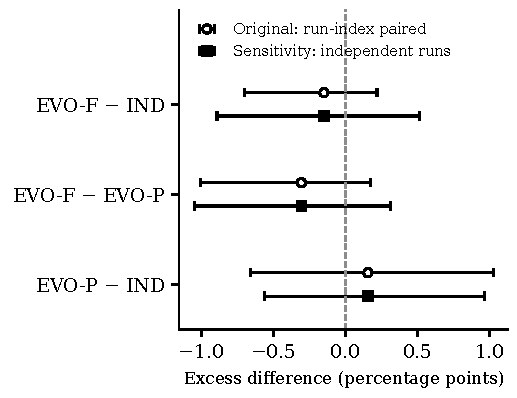
\includegraphics[width=\columnwidth]{figures/primary_bootstrap_sensitivity.pdf}
\caption{Primary and secondary contrasts under the original run-index-paired
bootstrap and the independent-run sensitivity. Both use paired graph indices,
five runs per strategy and 5,000 draws. Negative values favor the first
method; all intervals contain zero.}
\label{fig:transfer}
\end{figure}

\subsection{Synthetic Distribution Shifts}
\begin{table}[!htbp]
\centering\small
\setlength{\tabcolsep}{3pt}
\caption{Mean excess cost (\%) on synthetic shifts, each with 60 graphs.
Hub-cost variants share the primary topologies and cost multisets.
Size80 changes graph size; BA changes topology. Primary ID/random values
are in Table~\ref{tab:primary}. Negative values favor the method.}
\label{tab:shift}
\begin{tabular*}{\columnwidth}{@{\extracolsep{\fill}}lrrrr@{}}
\toprule
Method & Hub-exp. & Hub-cheap & Size80 & BA\\
\midrule
% Generated from saved JSON by scripts/reproduce_results.py.
IND & -0.378 & +0.302 & +0.213 & +0.065 \\
EVO-P & -0.579 & +0.548 & +0.294 & +1.322 \\
EVO-F & -0.615 & +0.093 & +0.168 & +1.438 \\
RS-PARAM & +0.827 & +0.129 & +0.401 & -0.349 \\
GR+P & +0.000 & +0.000 & +0.000 & +0.000 \\
RGR+P & -1.017 & +0.088 & -0.472 & -0.483 \\
Reverse-delete & +0.722 & +1.547 & +1.150 & +13.048 \\
\bottomrule

\end{tabular*}
\end{table}

Controlled cost--degree alignment changes performance
(Table~\ref{tab:shift}). All LLM strategies improve on greedy on average with
hub-expensive costs, yet the handcrafted RGR+P rule improves more.
Because topology and the cost multiset are fixed, this comparison concerns
cost allocation rather than cost scale.

On size and topology shifts, the LLM strategies lose to greedy on average.
RGR+P improves in both, while RS-PARAM improves only on BA. A useful
priority exists within the scaffold but is not consistently recovered by
evolution. Section~\ref{sec:rarity_form} analyzes its rarity weighting.

\subsection{Published T1/T2 Transfer}
\begin{table}[!htbp]
\centering\small
\setlength{\tabcolsep}{3pt}
\caption{External transfer: mean excess (\%) and median first-call runtime
(seconds, T1/T2). Each family has 24 weighted instances on shared topologies;
search methods use all five frozen winners. Timing describes the reference
interpreter. Full outcome counts and medians remain in the repository.}
\label{tab:external}
\begin{tabular*}{\columnwidth}{@{\extracolsep{\fill}}lrrr@{}}
\toprule
Method & T1 excess & T2 excess & \shortstack{Time\\T1/T2 (s)}\\
\midrule
% Generated from saved JSON by scripts/reproduce_results.py.
GR+P & +0.00 & +0.00 & 0.992/1.039 \\
RGR+P & -1.26 & -0.58 & 3.756/1.768 \\
Reverse-delete & +6.55 & +1.82 & 0.013/0.008 \\
IND & +0.18 & -0.08 & 4.011/2.881 \\
EVO-P & +0.20 & -0.03 & 4.104/2.954 \\
EVO-F & +0.40 & +0.16 & 3.842/2.628 \\
RS-PARAM & +1.60 & +0.80 & 8.377/5.257 \\
\bottomrule

\end{tabular*}
\end{table}

Frozen programs transfer without benchmark-specific tuning.
EVO-F has higher mean excess than IND and EVO-P in both weight families,
while RGR+P has the lowest (Table~\ref{tab:external}).
IND and EVO-P improve slightly on greedy under degree-dependent T2
weights; EVO-F does not. External family averages therefore show no
descriptive feedback advantage. Size/density rankings are mixed.

\begin{samepage}
RGR+P's gains are uneven: its wins/ties/losses against greedy are
11/11/2 on T1 and 7/15/2 on T2.\par
\end{samepage}

\begin{samepage}
All external solutions pass independent feasibility checks. CP-SAT certifies
only five T2 instances, all at $n=100$, and no T1 instance within its search
limit; exact-gap statistics on those five cases are not representative
of either full family.\par
\end{samepage}

\subsection{Classical Solver at 50 ms}
\begin{table}[!htbp]
\centering\small
\setlength{\tabcolsep}{3pt}
\caption{Same-session primary-graph control under a 50 ms end-to-end target.
Fixed methods have 180 measured calls and EVO-F 900. Late counts calls
exceeding the target; gaps and hits use certified optima.}
\label{tab:control}
\begin{tabular}{lrrrr}
\toprule
Method & Gap (\%) & Hits (\%) & Median ms & Late\\
\midrule
% Generated from saved JSON by scripts/reproduce_results.py.
GR+P & 2.89 & 66.7 & 4.17 & 0/180 \\
RGR+P & 3.37 & 63.3 & 10.50 & 0/180 \\
EVO-F & 3.21 & 63.3 & 14.94 & 0/900 \\
CP-SAT50 & 0.00 & 100.0 & 7.39 & 0/180 \\
\bottomrule

\end{tabular}
\end{table}

CP-SAT50 reaches every primary optimum in every repeat, with median
latency 7.39 ms versus 14.94 ms for EVO-F and no deadline overrun
(Table~\ref{tab:control}). On these original $n=40$ graphs, it offers both
better solution quality and lower median latency for the evaluated reference
implementation. This comparison concerns neither every possible optimized
learned heuristic nor the external benchmark's longer certification attempts.

Discovery used 800 attempts, yielding 513 novel-valid proposals within runs
and 287 invalid or duplicate proposals. The 600 LLM attempts cost
US\$0.0806 (IND), US\$0.1115 (EVO-P), and US\$0.1834 (EVO-F),
including unsuccessful and duplicate proposals. Recorded training solver
time was 58.2, 145.9, and 105.2 seconds, respectively; RS-PARAM used
323.6 seconds and no API calls. These totals include seed evaluations
but exclude reference setup, parsing, search overhead, and API waiting;
full evaluator wall time was not recorded. Discovery resources are
separate from the deployment runtimes above, which measure execution
of frozen heuristics.

\section{Analysis of Selected Heuristics}
\label{sec:selected}
\subsection{Why Do Final Solutions Converge?}

Across the five frozen EVO-F winners on the same 60 primary graphs,
construction orders differ from GR+P in 161 of 300 run--graph observations.
Only 61 have different pre-pruning vertex sets, 44 have different final
sets, and 23 have different final costs. Orders are compared as complete
sequences on the original labels; membership is compared as sets.
These are descriptive frequencies over dependent observations, not
300 independent graph samples.

The stages discard different kinds of variation. In 100 observations,
construction order changes without changing the constructed set.
Of the 61 different constructed sets, 17 converge to the same final set
after deterministic pruning. Another 21 observations retain different
final sets with equal cost. Thus, trajectory diversity exceeds
final-solution diversity, which in turn exceeds objective diversity.
Pruning explains one part of this convergence; selection during
construction and equal-cost alternatives explain the rest. A different
scoring expression can therefore produce many different choices without
improving the measured objective.

\begin{samepage}
\subsection{Why Does Rarity's Form Matter?}
\label{sec:rarity_form}

Seven of the 15 LLM winners are the greedy seed. Within EVO-F, runs 0
and 3 select that seed, while the other three select
\begin{equation}
\begin{aligned}
f_1 &= (g+0.4r)/q,\\
f_2 &= (g+0.55r)/q,\\
f_4 &= g/q+0.5r/q-0.2o.
\end{aligned}
\label{eq:selected_forms}
\end{equation}
\end{samepage}
The selected non-seed EVO-F programs therefore belong to a narrow
additive-rarity family, with an overlap penalty in run 4. This
characterizes the selected programs, not the full range of forms the
model could generate.

For the additive component, the bonus relative to coverage gain is
\begin{equation}
f(v,U)=\frac{g_v+\alpha r_v}{q_v},
\qquad
\frac{\alpha r_v}{g_v}
=\frac{\alpha r_v|U|}{k_v}.
\label{eq:rarity_scale}
\end{equation}
Coverage gain is normalized by the remaining demand $|U|$, whereas
rarity averages inverse neighborhood sizes over the $k_v$ newly covered
vertices. The relative bonus can therefore grow with $|U|$ or decrease
with $k_v$, even at the same average rarity. During construction, both
the uncovered set and the composition of each candidate's newly covered
neighborhood change. Graph size alone does not determine the bonus.

Multiplicative rarity has a different interpretation. Substituting the
feature definitions into Eq.~\eqref{eq:rarity} gives
\begin{equation}
\frac{g_vr_v}{q_v}
=
\frac{\bar c}{|U|}
\frac{1}{c_v}
\sum_{u\in N[v]\cap U}\frac{1}{|N[u]|}.
\label{eq:weighted_coverage}
\end{equation}
The leading factor is shared by all candidates at a step, so RGR+P
ranks vertices by total inverse-neighborhood weight of newly covered
demand divided by candidate cost. Standard greedy values each newly
covered vertex equally; RGR+P assigns more weight to demand vertices
with fewer possible covering neighbors. Additive rarity instead places
an average-rarity bonus alongside normalized coverage. It is not the
same weighted-coverage calculation.

\begin{table}[!htbp]
\centering\small
\caption{Interventions on all five frozen EVO-F winners. Mean excess
(\%) is relative to pruned greedy on training (30 graphs), primary and BA
(60 graphs each). No program is refit or reselected.}
\label{tab:ablation}
\begin{tabular}{lrrr}
\toprule
Intervention & Train & Primary & BA\\
\midrule
% Generated from saved JSON by scripts/reproduce_results.py.
Locked & -0.144 & +0.313 & +1.438 \\
$r=0$ & +0.209 & +0.200 & +0.049 \\
$o=0$ & -0.154 & +0.141 & +1.430 \\
No pruning & +6.922 & +7.558 & +10.642 \\
\bottomrule

\end{tabular}
\end{table}

\begin{samepage}
Table~\ref{tab:ablation} summarizes all five winners. For the three
non-seed winners, zeroing rarity changes training excess from
$-0.240\%$ to $+0.349\%$, primary excess from $+0.522\%$ to
$+0.334\%$, and BA excess from $+2.396\%$ to $+0.082\%$.\par
\end{samepage}

\begin{samepage}
The rarity term helps training fitness but its contribution does not
transfer to these held-out averages. Runs 1 and 2 reduce exactly to
greedy when rarity is zeroed; run 4 retains its overlap penalty.
Omitting pruning also worsens the five-winner averages, showing the
importance of the fixed scaffold.\par
\end{samepage}

RGR+P, by contrast, improves mean cost on BA and both external weight
families (Tables~\ref{tab:shift} and~\ref{tab:external}).
Together, the algebra and interventions make the functional form of
rarity weighting a plausible explanation for transfer differences.
They analyze the selected heuristics' behavior without establishing a
unique cause of the discovery policies' outcomes.

\subsection{Illustrative Decision Trajectories}

The following saved traces are the first qualifying primary improvement
and BA failure in lexicographic (run, instance) order. They illustrate
how scoring changes interact with construction and pruning.

\paragraph{A primary improvement.}
For primary instance 0014, run 1 uses $f_1$ from
Eq.~\eqref{eq:selected_forms}. At the third selection, vertices 15 and 35
both cover seven new vertices at cost two. Greedy selects 15 by ID;
the higher average rarity makes EVO-F select 35. EVO-F finishes at
cost 29, the certified optimum, versus greedy's 31. Vertex 35 is
itself pruned: its effect is on the subsequent construction trajectory,
rather than final membership. The strict improvement survives one of
ten saved vertex relabelings; the other nine tie greedy, showing the
example's sensitivity to ID-based tie-breaking.

\paragraph{A BA failure.}
For BA instance 0044, run 4 uses $f_4$.
It agrees with greedy for four selections, then chooses vertex 30
instead of vertex 19. Their new-coverage-to-cost ratios are 1 and 2,
respectively. The additive rarity term reverses this ranking even
with the overlap penalty; without rarity, the two candidates retain
greedy's ordering. Both trajectories later prune vertex 30.
Final costs are 34 for EVO-F and 33 for greedy, while RGR+P reaches
the certified optimum of 30. The first ranking reversal identifies a
departure that propagates through later choices; it does not isolate
the entire final loss to one decision. Complete traces and per-winner
summaries remain in the repository.

\section{Discussion and Limitations}

The proposal-policy comparisons do not establish a reliable held-out
improvement from parent conditioning or the additional prompt feedback.
EVO-P already uses fitness to select its archive; EVO-F adds numerical
summaries and case descriptors, after which parent histories can diverge.
The study therefore compares complete search policies, rather than
isolating the causal effect of numerical values in otherwise matched
prompts.

The frozen-program evidence is more specific about behavior than
discovery. Scoring changes often vanish before the objective is
measured; when they survive, rarity's functional form changes how
coverage is valued. This connects transfer to the representation,
but leaves archive conditioning and the training corpus as competing
explanations for which programs a policy selects.

The scope is limited by five runs per strategy, one shared training
corpus and a restricted DSL. Matched proposal attempts yield unequal
numbers of unique executable candidates. External evaluation covers
24 topologies under two weight regimes, with few certified optima;
T1/T2 change both cost magnitudes and their relationship to degree.
These constraints limit attribution and generalization. The
reference-implementation timings also leave open what optimized learned
heuristics and stronger large-scale classical controls would achieve.

\section{Conclusion}

The evaluated evolutionary policies do not establish a held-out advantage
over independent generation or a clear incremental benefit from the
prompt-feedback policy. Scoring diversity often produces trajectory
diversity without changing the final solution or cost. The form of
rarity weighting helps explain differences in frozen-program transfer,
while CP-SAT remains the stronger control on the original small graphs.
Broader representations and varied training corpora are needed to test
whether these search policies yield more useful deployed heuristics.

\section{Reproducibility}

Source code, configurations, selected heuristics and numerical results
are available in the accompanying repository. The README gives commands
for reproducing tables and analyses from saved observations without LLM
calls; \nolinkurl{scripts/analyze_selected.py} derives the winner-level
mechanism summaries. The original environment is Python 3.12.7 on
Windows 11, NetworkX 3.7, OR-Tools 9.15.6755, NumPy 2.5.4 and Matplotlib
3.11.2.

\subsection*{Generative AI disclosure}
Generative AI tools were used to support literature exploration, implementation, debugging, experimental analysis, and manuscript preparation. They also served as discussion aids for methodological decisions. The LLM used for heuristic generation is described separately in the methodology. The author reviewed the AI-assisted work and takes responsibility for the final results and manuscript.

\begingroup\raggedright\urlstyle{same}
\interlinepenalty=10000
\balance
\bibliographystyle{unsrt}
\bibliography{references}
\endgroup
\end{document}
